\documentclass[12pt]{article}

\usepackage{amssymb}
\usepackage{booktabs}
\usepackage{floatrow}
\usepackage{graphicx}
\usepackage{url}

\title{Project}
\date{2015-09-18}
\author{Eric Scott Freeman}

\begin{document}
	\pagenumbering{gobble}
	\maketitle
	\newpage
	\tableofcontents
	\newpage
	\pagenumbering{arabic}
	\section{Introduction}
		
	\section{Related Work}
		Unfortunately software plagiarism is a problem both in the classroom and in the workplace. A number of applications have been created to help detect this problem. While these tools can detect similarities in programs, the flagged files must still be manually examined to determine whether or not code was plagiarized.
		
		There are several different general techniques that are used to look for plagiarism. The tools analyzed in this project used either fingerprinting or stylometry.
	
		\subsection{Fingerprinting}
			Several tools use a technique called fingerprinting to detect plagiarism. In fingerprinting algorithms, hashes of $n$-grams, substrings that are $n$ characters, are saved and compared to help find plagiarism. Not all hashes are stored due to the large number that would be produced. 
		
			\subsubsection{Winnowing}
				Moss uses a technique called winnowing to select which hashes to save \cite{schleimer+wilkerson+aiken}. In the winnowing algorithm, a window, selection of contiguous hashes, is used to help select which hashes to save. The smallest hash from a window is saved, and then the window moves one hash over. The smallest hash from the next window is often the smallest hash from the previous window. If so it is not saved again. Figure \ref{fig:winnowing1} shows an example of how winnowing works. The orange box represents the shifting window. The green box shows whenever a new hash is saved.
				
				\begin{figure}[h!]
					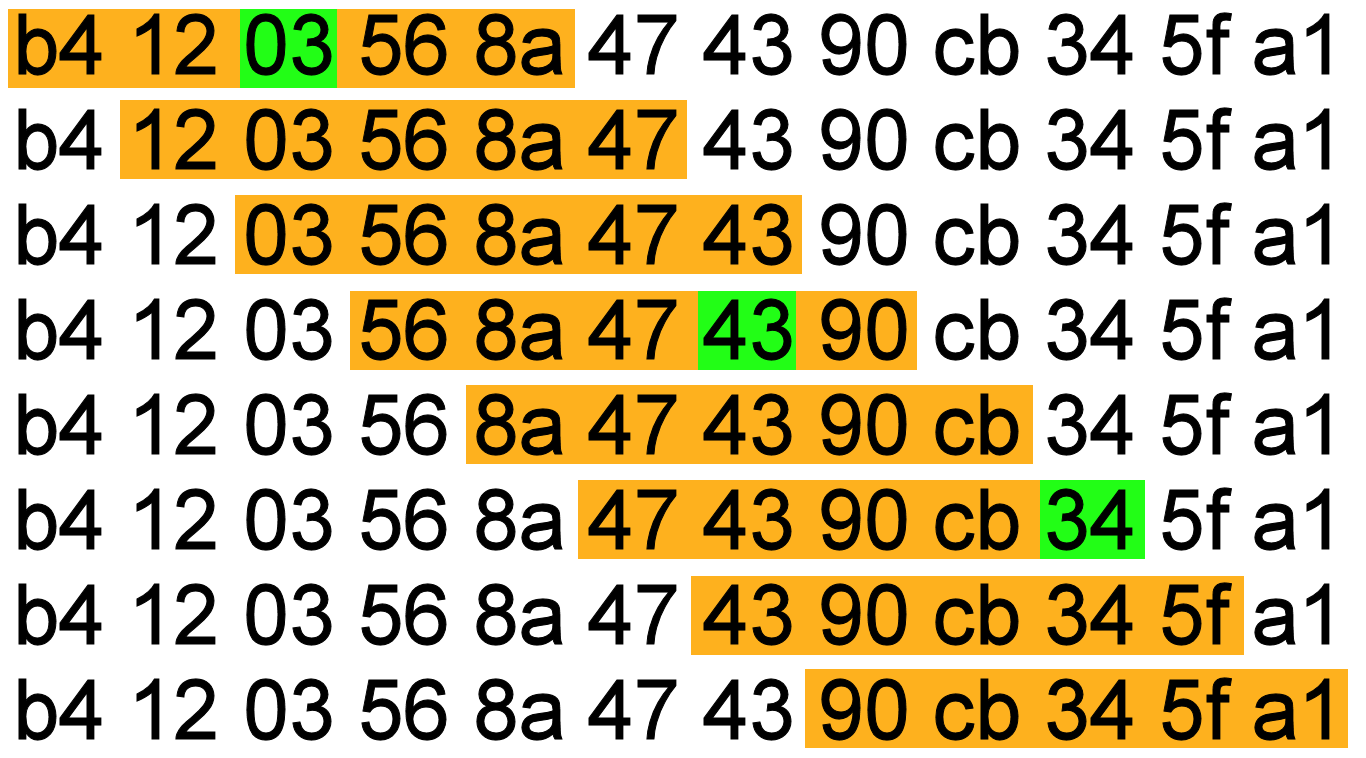
\includegraphics[scale=0.75]{Winnowing.png}
					\caption{Winnowing.}
					\label{fig:winnowing1}
				\end{figure}
			
			\subsubsection{Running-Karp-Rabin Greedy-String-Tiling}
				JPlag uses Running-Karp-Rabin Greedy-String-Tiling (RKS-GST) to compare hashes of code in plagiarism detection \cite{prechelt+malpohl+philippsen}. RKS-GST was originally used in YAP3, another plagiarism detection tool. In RKS-GST, the Greedy String half of the algorithm forms pairs of substrings, each from a different string. Then the Karp-Rabin half of the algorithm hashes each substring in the pair \cite{wise}. This is done to help detect code reordering.
		
		\subsection{Stylometry}
			Another approach is to use code stylometry, which analyzes the style of writing or coding.
			
			\subsubsection{Abstract Syntax Trees}
				Caliskan-Islam, et al. use abstract syntax trees (ASTs) to compare the styles of authors \cite{caliskan-islam+harang+liu}. Things that are easily changed in code, such as variable names, become leaves in the AST, while the structure of the tree is harder to change \cite{caliskan-islam+harang+liu}. Figure \ref{fig:ast} shows an abstract syntax tree of the code in Figure \ref{fig:astcode}. Note how the leaves, or circular nodes, in Figure \ref{fig:ast} are variable names, constants, and a function name.
				
				Michal Bohuslávek's dupl application uses ASTs to find similarities in code \cite{bohuslave}. It looks for any copies of code, not just plagiarism. So if a piece of code is duplicated even in the same file, it will test positive.
			
				\begin{figure}
					\begin{floatrow}
						\ffigbox{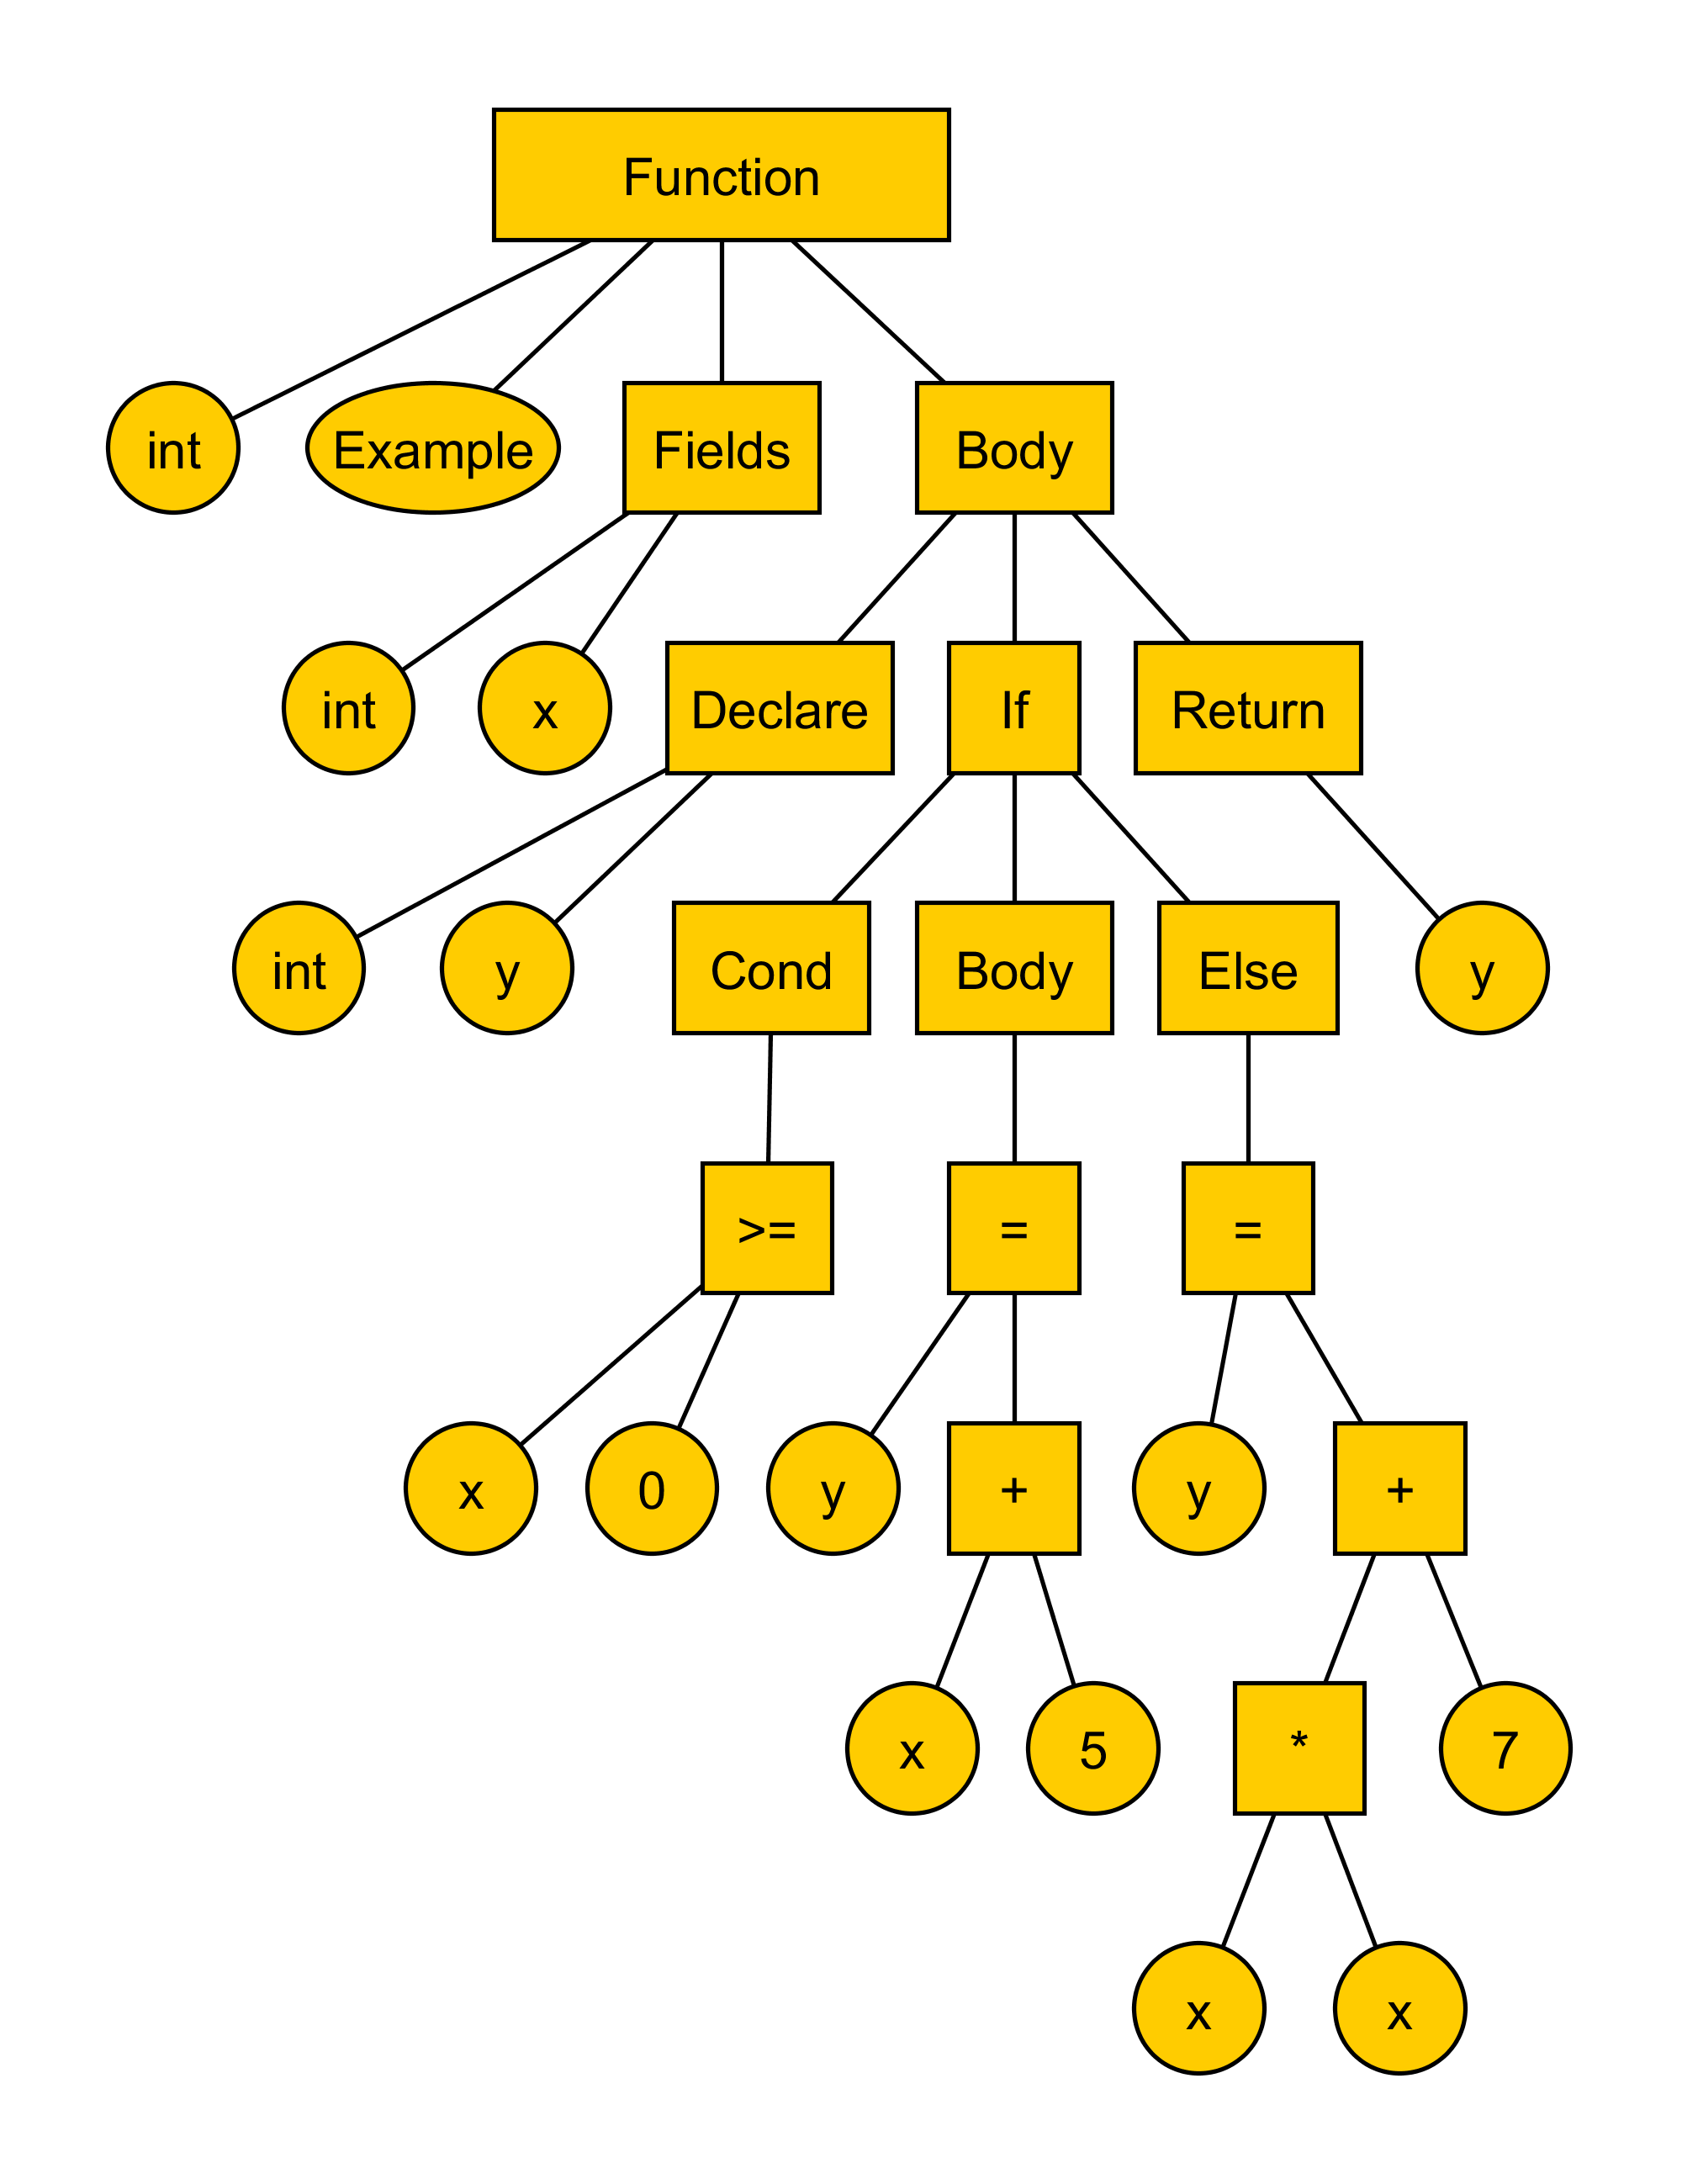
\includegraphics[scale=0.1]{AST.png}}{\caption{Abstract syntax tree.}\label{fig:ast}}	\ffigbox{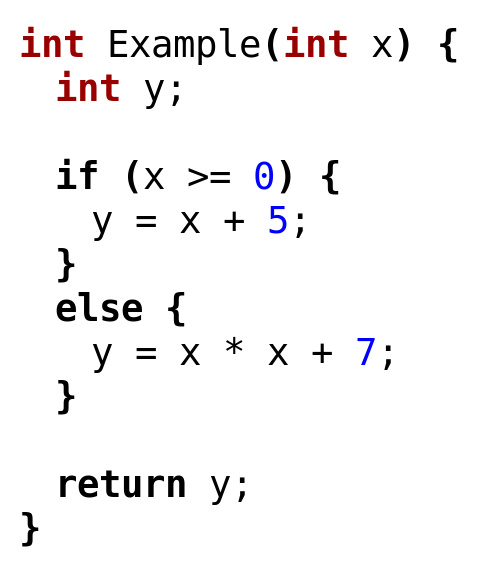
\includegraphics[scale=0.5]{ASTcode.png}}{\caption{Example code.}\label{fig:astcode}}
					\end{floatrow}
				\end{figure}
		
		\subsection{Supported Languages}
			Fingerprinting and string comparison techniques can be used to analyze source code written in languages other than their officially supported languages. Moss can analyze Go code, even though it is not technically supported. Since ASTs need to parse the code, applications which use them are stricter on which languages they can analyze. For example dupl only supports code written in Go. Table \ref{tab:languageSupport} shows the languages officially supported by several anti-plagiarism tools.
		
			\begin{table}[h!]
				\begin{center}
					\caption{Officially supported languages by various tools}
					\label{tab:languageSupport}
					\begin{tabular}{ccccccccccccccc}
						\toprule
						Tool & Java & Go & C & C\verb!++! & C\verb!#! & Python & Perl & others\\
						\midrule
						Moss & \checkmark & & \checkmark & \checkmark & \checkmark & \checkmark & \checkmark & \checkmark \\
						JPlag & \checkmark & & \checkmark & \checkmark & \checkmark & & & \checkmark\\
						Plaggie & \checkmark & & & & & & & \\
						SIM & \checkmark & & \checkmark & & & & & \checkmark\\
						dupl & & \checkmark & & & & & & \\
						\bottomrule
					\end{tabular}
				\end{center}
			\end{table}
		
	\section{Design}
	\section{Results}
	\section{Analysis}
	\section{Conclusion}
	\bibliography{sources}
	\bibliographystyle{ieeetr}
\end{document}